\section{Literature review} 


\subsection{TimeGPT-1 \cite{garza2023timegpt}}

TimeGPT-1 is closed-source model - meaning that there is a lot of opacity to model's architecture, parameters and trainng data.

\subsubsection{Architecture}

TimeGPT-1 has encoder-decoder structure with multiple layers, each having residual connections and layer normalization. It utilizes self-attention mechanism based on the original Transformer \cite{vaswani2017attention}. 

Special capability of TimeGPT-1 is multivariate time-series forecasting - meaning that it is able to take into account "special events" and exogenous features\footnote{Special events and exogenous features are time-series which are assumed to have some influence on the target time-series. Example of the former being bank holidays if the target time-series if number of flights per day and example of the latter being price of petrol if we are forecasting number of cars on the road.} when making predictions on a target time-series. However, in order to take full advantage of this feature, we would have to know for certain the realizations of the exogenous variables in the future which is almost never the case in time-series forecasting\footnote{because we can never predict anything in the future with certainty.}. TimeGPT-1 solves this by separately forecasting the exogenous variables into the future and then basing the forecast of the target time-series on its own forecast of the exogenous features. %In my opinion this is a flawed approach, inferior to simple uni-variate prediction as it brings in additional dimensions of uncertainty - whether the exogenous variables forecast are correct and whether the forecasted relationship between exogenous variables and target time-series is correct. One could make a case that 

\subsubsection{Training Data}

Authors claim TimeGPT-1 has been trained on a data-set containing over 100B data-points - the largest collection of publically availible time-series according to their knowledge. Data comes from the domains of finance, economics, demographics, healthcare, weather, IoT sensor data, energy, web traffic, sales, transport, and banking. Due to diversity of data domains, the training set contains time-series with many different characteristics: seasonalities, cycles, trends, noise, outliers. Having been trained on such a diverse dataset, TimeGPT-1 has very strong robustness and generalization capabilities.

\subsubsection{Results}



\subsection{Lag-Llama \cite{rasul2023lag}}

\subsubsection{Tokenization}

Lag-Llama constructs "lagged features" from the past values of the time-series according to a set of frequency-dependant set of lag indices L\textsubscript{indices}={1, ..., N}. The set of lagged features of a point x\textsubscript{t} at timestamp t is then \{x\textsubscript{t-L\textsubscript{indices}[i]}, for all integers i such that 0<i<N+1\}. Lag-Llama also constructs "date-time features" F which for a point x\textsubscript{t} in time t contain information about second-of-the-minute, minute-of-the-hour, ..., month-of-the-year. Final tokenization is done by simply concatenating the date-time features and lagged features into a single vector.

\subsubsection{Architecture}

Lag-Llama is an open-source, decoder-only TSFM based on LLaMA \cite{touvron2023llama} architecture with reduced number of parameters\footnote{ Original LLaMA series comes in sizes of 6.7B, 13.0B, 32.5B and 65.2B parameters.} (2.5m) . Similarly as LLaMA, Lag-Llama utilizes concepts such as RMSnorm \cite{zhang2019root}\footnote{RMSnorm is a layer normalization technique. Zhang and Sennrich (2019) demonstrate that centering component of the LayerNorm technique is dispensable (and computationally expensive) and propose their own layer normalization strategy called RMSnorm which delivers similar benefits (more stable training and better model convergence) but with lower computational cost.}, RoPE \cite{su2024roformer}\footnote{RoPE stands for Rotary Positional Encoding. This is a method for positional encoding. RoPE enables valuable properties, including the flexibility of sequence length,
decaying inter-token dependency with increasing relative distances, and the capability of equipping linear self-attention with relative position encoding.} and SwiGLU \cite{shazeer2020glu}\footnote{SwiGLU activation function is a combination of swish and GLU activation functions. With beta hyperparameter equal to 1, it is of similar shape as ReLU but completely smooth (continuous) - therefore "behaving better" during model training.} activation function\cite{miller2024survey}. On top of N decoder layers, Lag-Llama has a "parametric distribution head". Parametric distribution head is a module which predicts the distribution parameters of the next prediction, given the set distribution. Authors of the paper have chosen student-t distribution for the distribution head, meaning that at inference time, the model predicts the degrees of freedom, mean and scale \cite{student1908probable} of the t-distribution from which it randomly draws n samples - idea being that this sample of n predictions gives a probabilistic insight into the model's prediction. See Figure \ref{fig:lagllama}:

\begin{figure}[h]
\centering
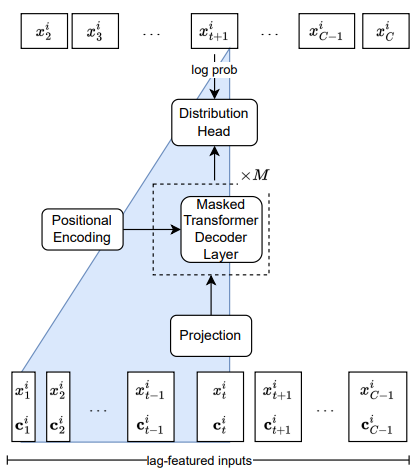
\includegraphics[width=8cm]{Image/lag_llama.PNG}
\caption{Lag-Llama architecture \cite{rasul2023lag}}
\label{fig:lagllama}
\end{figure}

\subsubsection{Training data}

Lag-Llama is pre-trained on diverse set of time-series domains such as energy, transportation, economics, nature, air quality and cloud operations.